\documentclass[final]{cmpreport}
\title{Population Dynamics}
\author{Edward Sleightholme}
\ccode{First Draft Report}
\registration{100137423}
\supervisor{Christopher Greenman}
\usepackage{rotating}
\usepackage{subfloat}
\usepackage{titlesec}
\usepackage{pgfgantt}

\usepackage{natbib}
\usepackage{hyperref}

\graphicspath{ {images/} }
\summary{
	Populations that are encountered on a daily basis by most of us. This report is to study these populations and there dynamics to see if there are any common trends that can be identified and studied. This will be done using both mathematical models and computer simulations. 
	
	The the effects single populations have on themselves are be explored. Also several types of relationships between populations are explored.This is done with the goal of finding general dynamics and trends that crossover multiple popualtions.
	
	This paper looks at single popualtions, the effect of of competition on a popualtion, the effects of predator prey relationship and many other population dynamics}
\acknowledgements{I would like to thank Christopher Greenman my project supervisor for his continued support for this project}
\begin{document}

\section{Introduction}
Populations are a important topic to understand as they are something dealt with on a regular basics. Whether studying about bacteria on a  Petri dish or trying how predict how a city will change over time. If you are able to find and understand common trends in populations you can predict how most populations will react under certain conditions. This information can be very important and helpful for many subjects from city planning to biology. The main goal of population dynamics is to find and define and explain trends in populations.Finding and exploring these trends is the main goal of this paper.

\subsection {Defining a population}
A population can be defined as a group of similar individuals usually of the same species. With this definition you can get many different types of populations. You can get populations that are easily defined. These populations tend to be isolated populations with no immigration or emigration.With easy to measure and see behaviours. You can also get hard to define populations. These tend to be the opposite of the populations before with them having lots of immigration and emigration and have hard to measure/understand behaviours . These types of populations are hard to study and understand. But if you can find trends within easy to define populations they may also appear in hard to define populations meaning you can get a insight in to the way that these populations work and function.

Also populations can also divided in to 2 other groups. These groups are continuous and discrete populations. Continuous populations are populations what breed or react in a continuous manner meaning that they can breed and react at any time . Were as discrete populations breed and react in discrete units of time. These 2 types will be explored later in the paper.

\subsection {Features of a Population}

A population is defined by its features. These features can encompass many things from the number of individuals are in the population to or the birth rate of the population. These features can be categorized mostly in to 3 groups.

\subsubsection{Individual Features}
Firstly there are features that relate to an individual. These features  include gender, age, health and many other features that only affect a single individual of a population. These types of features tend to show the finer details of a population. But in practice it is very hard to keep track of lots of these features due to the vast number of them as every member of the population will have them making it hard to keep track of them all.

\subsubsection{Subset Features}
Secondly there are features that make up a subset of a whole population. These subset features for example could be death rates at certain age ranges or birth rates within certain areas of a environment the population is in. These subsets can become increasing complex and can also become difficult to measure and keep track of.

\subsubsection{Whole population Features}
Thirdly there whole population features these features are about the population as a whole. This could be the number of individuals there are in the population or a general density of the population. These features are very good at showing how the population is doing in several simple number. The issue with just using these features is that you will lose a lot of the details about how the population acts.

\subsection{Abstraction of a Population}
There are countless features a population can have and keeping track off them all is a pointless task. This would lead to having to do a high amount of work for very little gain. If you were to narrow down these features you have about a population them it becomes easier to analysis the data you have and so it becomes easier see trends in the data. 

Usually the most important features to measure about a population is the amount of individuals you have in a population and the features that directly affect this number (Eg Birth rate,Death rate, etc.). This is because usually the success of a population comes from the number individuals a population has and the rate this number changes at.

\subsection{Importance of Dynamics of a Population and how to show understand them}

The dynamics of a population are the finding the biological and environmental processes that affect a population and finding way to express them mathematically. These can be very important as if they can be used to explain trend in one population then they can be easily applied to other populations to see if the populations are similar. 

There are many ways to show get these dynamics.Below are listed 3 ways to gather these dynamics

\subsubsection{Field Work}
The most common way to gather data is to go to the location of the population and manually measure various features you wish to gather about a population. This method is very good if the population is readily available as there is it very hard to get data wrong. The downside of this is it can be quite time consuming and only provide data about the population at the time the field work occurs. 

Also if the population does not exist yet (for example you are planning on introducing a species to a location) or you are trying to predict the future for a population this method does not work. 

\subsubsection{Mathematical Models}

Mathematical models are a important way of explaining trends in a population. They are most useful if you already have a basic understanding of populations dynamics. They can be used to explain trends within data you already have in a population and to test out theories about population dynamics. They can also achieve what field work can not which is to predict the future for a population and attempt to show trends for populations that do not exist yet. 

These models can be tested by comparing them against data the collected using field work. This enables the models to be validated and a confirmed as correct.The disadvantages of this type of model is that for certain more complex behaviours can become very hard to design mathematically.

\subsubsection{Simulations}
Another useful tool to use is design and make a simulation.This method is similar to the mathematical method in terms of results and data needed to start designing a simulation. This method unlike a mathematical model enables you to show complex behaviour. Also it is possible to see emergent behaviour with in a population using a simulation rather than a mathematical model. 


\section{General Overview of Simulations used}
Over the course of this paper simulations will be used to demonstrate  trends and features common in many populations.  These simulations will be used to cross reference against the results of the mathematical models made. This will enable us to see similarities and differences between the two ways of showing populations in this paper.


\subsection{General assumptions made on all simulations in this paper}

All simulations in this paper will be built in a similar way. Firstly all the simulations will be on a 2d grid and each cell of the grid will be only able to hold one individual at a time. This is because it will make the rule sets of each simulation easier to express and understand. Also it will make it easier to display a visualisation of the simulation.

Secondly all simulations will have there edges loop around to the opposite side. This will occur so that every cell in the simulation will have the same amount of sides next to it. This is to stop errors from occurring at the edge of each simulation.

\subsection{Simulations Technical}

All simulations made will be made using the programming language python (\cite{python}). This is because python is a light weight easy to use language that can run quickly and efficiently. The simulations will visualised using the python import pygame (\cite{pygame}). This is used to visualise the simulations made so that they can be easily analysed and understood.
	
	
\section{Single Populations}
	
	Single populations are the best place to start when exploring trends in populations. This is because they don't have to deal with the factors of other populations interacting with them. This lets us see the factors that influence a single population. Also it provides a good starting point for building up to multiple populations models.
	
	\subsection{Density Independent Models}
	
	Density independent models are models that assume certain things about a population. Firstly there is no immigration/emigration in the population. This means that only births and deaths control the size of a population. The second assumption to make is that all individuals are able to reproduce instantly and spontaneously without need of any other member of the population. This like assumption like one made before it enables the simplification of the mathematical models made. Thirdly it is assumed that there are no limiting factors on a population including limitations such as space or food.
	
	Density independent models can be split in to two types. Models that describe discrete populations and those that describe continuous populations.
	
	\subsubsection{Discrete Populations}
	
	A discrete population is a population in which each generation as a discrete group. This means a population that has non-overlapping generations. This is typical for animal populations such as butterflies . So for these populations it is best to measure time in units of generations and these timeunit will be denoted as $t$. The number of individuals in the next generation with relationship to the current generation will be denoted as $R$. So setting $N_t$ as the number of individuals in a population at generation $t$ the formula below is formed.

	\begin{equation}
		N_{t+1}=RN_t
	\end{equation}
	
	Equation (1) can be manipulated to get $N_t$ in terms of $N_0$

	\begin{equation}
		N_{2}=RN_1=R(RN_0)=R^2N_0 
	\end{equation}
	
	\begin{equation}
		N_t=R^tN_0 
	\end{equation}
	From equation number 3 it can be seen that the population will grow or shrink at an exponential rate. This is proven by plotting this on a graph.
	
	\begin{figure}[h!]
	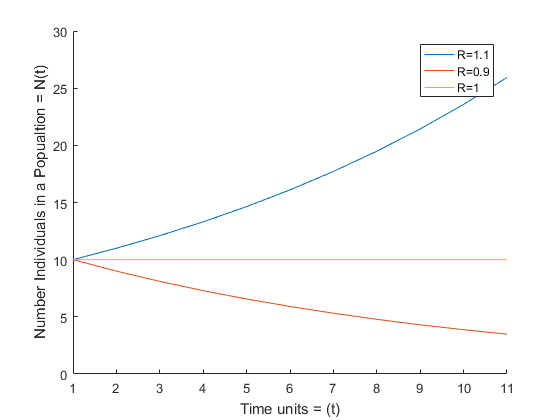
\includegraphics[width=\textwidth]{SingleDiscetePopulationsGraph.png}
		\caption{Example of equation (3) where $N_0 = 10$ with varying values of R}  
	\end{figure}
	
	
	
	From Figure 1 these conclusions can drawn about $R$ 
	\begin{itemize}
		\item $R > 1$ the model will increase expectationally forever
		\item $R = 1$ the model will stay constant
		\item $R < 1$ the model approach 0
	\end{itemize}
	
	\subsubsection{Continuous Populations}
	
	A continuous population on the other hand is a type of population that breeds continuously such as rabbits,humans or dogs. This leads to over lapping generations. This means a new model must be produced as the previous model is inappropriate for continuous populations. $t$ shall be changed from the number of generations to a value of arbitrary time units. Also the number of individuals in the population will be denoted as $N(t)$. The values $t$ and $N$ will not be limited to integer values even though you can not get half of a member of a population as this is a suitable approximation needed for this type of model. Also need is the chance of a birth by an individual $b$ and chance of death for an individual $m$. Also denoted is rate of change in the total number of individuals $\frac{dN}{dt}$. The rate of birth will be denoted as $bN$ and rate of death $dN$. This will show rate of change as the rate of births minus the rate of deaths. This leads to the equation 
	\begin{equation}
		 \frac{dN}{dt} = bN-mN
	\end{equation}
	This is normally written as  
	\begin{equation}	
		\frac{dN}{dt} =rNt
	\end{equation}
	Where 
	\begin{equation}
		b-m = r 
	\end{equation}
	
	$r$ shows the rate of change within a population. Now $N(t)$ is needed to be received as a function of $t$. So starting with
	\begin{equation}
	\frac{dN}{N} =rdt
	\end{equation}
	Integrate equation from $t=0$ to $t=T$
	\begin{equation}
	 	\int_{t=T}^{t=0}\frac{dN}{N} =\int_{t=T}^{t=0}rdt
	\end{equation}
	Compute integrals of the equation
	\begin{equation}
	 	\ln(N(t))|^{t=T}_{t=0} = rT|^{t=T}_{t=0} 
	\end{equation}
	Evaluate the equation
	\begin{equation}
	 	\ln(N(T)) - \ln(N(0)) = rT 
	\end{equation}
	Get exponential of both sides
	\begin{equation}
	 	\exp^{\ln(N(T))}\exp^ {- \ln(N(0))} = \exp^{rT} 
	\end{equation}
	Then solve to get $N(T)$
	\begin{equation}
	 \frac{N(T)}{N0}= \exp^{rT} 
	\end{equation}
	\begin{equation}
	 N(T)= N(0) \exp^{rT} 
	\end{equation}
	
	Graphing equation (13) you get the graph seen in figure 2. From this graph these conclusions can be drawn
	
	\begin{figure}[h!]
		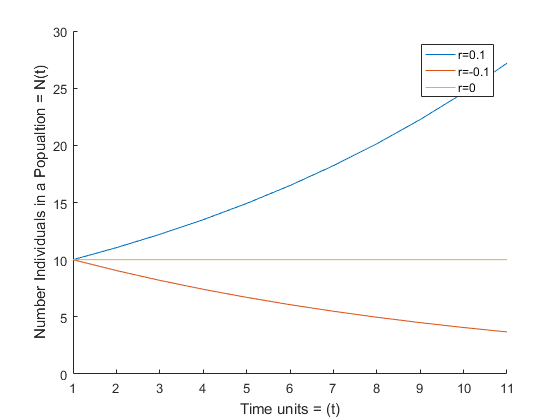
\includegraphics[width=\textwidth]{SingleContinousPopulationGraph.png}
		\caption{Example of equation (13) where $N_0 = 10$. With varying values of $r$}  
	\end{figure}
	
	\begin{itemize}
		\item $r > 0$ the solution will increase expectationally forever
		\item $r = 0$ the solution will stay constant
		\item $r < 0$ the solution approach 0
	\end{itemize}

	As you can see these are similar conclusions as the ones received from equation (3).Concluding from this it can be assumed that discrete and continuous populations share a common trend.
	
	\subsubsection{Common trends in Density Independent Models}
	
	As before stated discrete and continuous populations share a common trend. As both types of populations produced almost identical density independent models. The equations between continuous and discrete models can be combined to form the equation .
	\begin{equation}
	 R= e^r 
	\end{equation}
	If R is close to one or r is little it can be approximated using Taylor's series.
	\begin{equation}
	 R \approx 1+r 
	\end{equation}
	From this it is proven that the both equation (13) and (3) show similar behaviour and then so does discrete and continuous populations.
		
	The clear common trend is that both models display exponential growth or a sharp drop to 0 population. The exponential growth can be explained due to the fact that the populations with out limitations will just keep breeding. This has been proven in the real world by cases such as bullfrogs being introduced to Australia. In this case the population has grown exponentially due to a lack of environmental and predatory limiting factors being applied to them. 
	Also the sharp tend towards 0 can be explained by understanding that if a animal is introduced in to a unfavourable environment such as a tiger being put on the north pole it will quickly die out.
	
	From these conclusions it be assumed that even though these 2 models are simplistic in nature they show important trends that are common in many populations. Namely that populations with out limitations will either grow exponentially or exponentially drop towards 0.
		
	
	\subsubsection{Age Structures}
	
	The previous models ignored several important factors. The one that be will add in now is age. Age effects all aspects of an individual. Firstly many long lived species such as elephants or tortoise don't reach maturity until they are 15 or 18 years in to there lives. This means that the chance of breeding changes as a result of a change of age. Also the survival of a individual changes by what age they are for example frogs lay between 1,000 and 2,000 eggs at time of breeding yet only around five will become fully matured frogs with many dying before they reach full maturity . From this it can assumed the chance of death of a individual in a population changes over time. This means age is a important factor to take in to account when understanding a population.
	
	
	For discrete populations it is simple enough to make models to show age structures. The simplest population to model and the population that will be used in this paper will be to model population that only has 2 generations alive at a time. Again $t$ will be denoted as a the time between generations and for this example the time unit $t$ will be denoted as years. So $n_0(t)$ will be the total number of 0 year-old at time $t$  and $n_1(t)$ as the total number of 1 year-old at time $t$. So the total number of individuals in a population will be defined as $N(t)$ this means that.
	
	\begin{equation}
	N(t) =n_0(t)+n_1(t) 
	\end{equation}
	
	Each generation of the population will need a separate birthrate this will be denoted as $b_0$ for birth rate for the group $n_0(t)$  and  $b_1$ for the birth rate of the group  $n_1(t)$. Finally there need to be a survival rate for 0 year-olds becoming 1 year-olds this will be denoted as  $S_0$. There is no need for a survival rate for 1 year-old individuals of the population as it will be assumed that all 1 year-old individuals will die before they can become 2 years old. These assumption lead to the equations.
	
	\begin{equation}
	 n_0(t+1) = n_0(t)b_0 + n_1(t)b_1
	\end{equation}
	\begin{equation}
	 n_1(t+1) = n_0(t)S_0
	\end{equation}
	
	Next from the equations above a question can be asked does adding a age structure still make the previous model $N_{t+1}=RN_t$ correct. This model depends on $R$ being a constant value and that the population will grow at a exponential rate. This at first looks like it is satisfied by the equations above as the population will increase at a exponential rate as can be seen in Figure 3. But as looking at table 1 it can seen that changing the starting ratios of the ages of the model causes the population to grow at different rates. This means $N_{t+1}=RN_t$ is not true for this model.
	
	\begin{figure}[h!]
		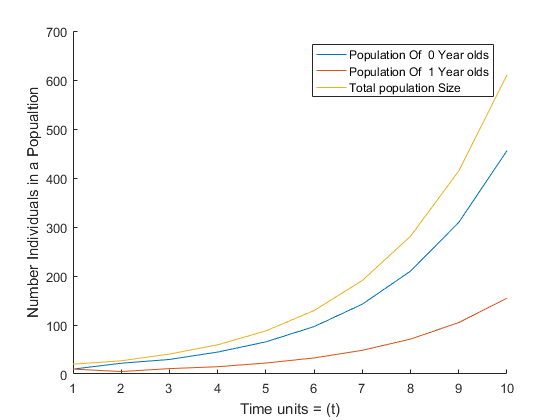
\includegraphics[width=\textwidth]{ageStructure.png}
		\caption{Graph shows a 2 generation age structured population as shown in equations (17) (18). With the starting conditions $n_0(0) =10$,$n_1(0) =10$  , $b_0 = 1.1$ , $b_1 = 1.1$ , $S_0=0.5$. This graph shows the population grows at a exponential rate}
	\end{figure}

	\begin{table}[h!]
	\centering
	\caption{Table showing affects of changing the start conditions of the equations (17) (18) and the effects it has on the growth of the populations}
	\begin{tabular}{|l|l|l|l|l|}
		\hline 
		$n_0(0) $ & $n_1(0) $ & $N(0) $ & $N(10)$ & $N(20)$ \\
		\hline
		0       & 20                                      & 10                               & 521                               & 25149      \\                  
		5       & 15                                      & 20                               & 566                               & 27283      \\                     
		10   	& 10                                      & 20                               & 610                               & 29417      \\                       
		15  	& 5                                       & 20                               & 654                               & 31550      \\                    
		20      & 0                                       & 20                               & 699                               & 33684      \\     
		\hline                 
	\end{tabular}
	\end{table}
	
	One way to get a steady growth rate though is to keep the ratio of 1 year-olds to 0 year-olds the same. This then enables the growth rate of the population to stay the constant for different ratios of starting ages in the population. So lets assume
	
	\begin{equation}
	 cn_0(t) = n_1(t)
	\end{equation}
	
	Where $c$ is the ratio between the number of 0 year-olds and 1 year-olds. This can substituted in to equations (17),(18) to get
	
	\begin{equation}
	 n_0(t+1) = n_0(t)b_0 + cn_0(t)b_1 
	\end{equation}
	
	\begin{equation}
	cn_0(t+1) = n_0(t)S_0
	\end{equation}
	
	Then making $n_0(t+1)$ be subject
	
	\begin{equation}
	n_0(t+1) = \frac{ n_0(t)S_0}{c}
	\end{equation}
	
	\begin{equation}
	 n_0(t)b_0 + cn_0(t)b_1 =\frac{ n_0(t)S_0}{c}
	\end{equation}
	
	divide by $n_0(t)$
	
	\begin{equation}
	 \frac{S_0}{c} = b_0 + cb_1 
	\end{equation}
	
	make subject = 0 
	
	\begin{equation}
	 0 = c^2b_1+ cb_0 -S 
	\end{equation}
	
	Using quadratic equation to solve
	
	\begin{equation}
	 c=\frac{-b_0\pm\sqrt{b_0^2-4S_0b_1}}{2b_1}   
	\end{equation}
	
	The variable $c$ can be solved to be 2 possible values. If $c>0$ then a positive ratio happens  and if $c<0$ a negative ratio happens. From equation (24) it can be seen that the growth rate of the population is $\frac{S_0}{c} $. So a positive $c$ makes this a possible growth rate of a population. But what if the populations age structure does not start at this ratio.
	
	
	\begin{table}[h!]
		\centering
		\caption{Table showing the change in the  ratio between  $n_0(t)$ and  $n_1(t)$ over $t$}
		\begin{tabular}{|l|l|l|l|l|}
			\hline
			$t$  & $n_0(t)$  & $n_1(t)$  & $N(t)$       & ratio between  $n_0(t)$ and  $n_1(t)$    \\
			\hline
			1  & 10          & 10          & 20          & 1           \\
			2  & 22          & 5           & 27          & 4.4         \\
			3  & 29.7        & 11          & 40.7        & 2.7         \\
			4  & 44.77       & 14.85       & 59.62       & 3.014814815 \\
			5  & 65.582      & 22.385      & 87.967      & 2.92972973  \\
			6  & 96.7637     & 32.791      & 129.5547    & 2.950922509 \\
			7  & 142.51017   & 48.38185    & 190.89202   & 2.945529574 \\
			8  & 209.981222  & 71.255085   & 281.236307  & 2.946894555 \\
			9  & 309.3599377 & 104.990611  & 414.3505487 & 2.946548599 \\
			10 & 455.7856036 & 154.6799689 & 610.4655724 & 2.946636251 \\
			\hline
		\end{tabular}
	\end{table}
	
	In table 2 the ratio will always tends towards the ratio of age distribution calculated . This means $c$ will be defined as the stable age distribution as all other age ratios all others tend towards this ratio. Also as the ratios tend towards $c$ but do not equal $c$ it is possible to see if a populations ratio has been disturbed in its past. 
								
	There is a far better way to display equations  (17) and (18) is as matrices. Below is the way the above equations can be expressed as matrices.
	
	\begin{equation}
	\begin{pmatrix} 
	b_0 & b_1 \\ 
	S_0 & 0  \\ 
	\end{pmatrix}  \begin{pmatrix} 
	n_0(t) \\ 
	n_1(t) \\ 
	\end{pmatrix} = \begin{pmatrix} 
	n_0(t+1) \\ 
	n_1(t+1) \\ 
	\end{pmatrix}
	 \end{equation}
	
	As before it will be assumed that the ratio between the number of 0 year-olds and 1 year-olds is constant. In previous models growth was shown as $\frac{S_0}{c} $ but now it will be denoted as $\landa$. This type of stable ratio between different ages in a population is called a stable age distribution. The stable age distribution is tended to towards by other age distributions.
	
	Stable age distribution can be displayed as matrices. 
	\begin{equation}
		\begin{pmatrix} 
		b_0 & b_1 \\ 
		S_0 & 0  \\ 
		\end{pmatrix}  \begin{pmatrix} 
		n_0(t) \\ 
		n_1(t) \\ 
		\end{pmatrix} = \begin{pmatrix} 
		\lambda n_0 \\ 
		\lambda n_1 \\ 
		\end{pmatrix}
	\end{equation}
	
	 Because of one of first to describe this was P.H Leslie (\cite{leslie})  so this	
	 $\begin{pmatrix} 
	 b_0 & b_1 \\ 
	 S_0 & 0  \\ 
	 \end{pmatrix}$  this be called a Lesile Matix and denote it by $L$ also $N$ will be denoted as a vector of total population size.
	 
	 \begin{equation}
	N = \begin{pmatrix} 
	 n_0(t) \\ 
	 n_1(t) \\ 
	 \end{pmatrix}
	\end{equation}
	
	So from this the equation below can be made.
	\begin{equation}
	LN= \lambda N 
	\end{equation}
	\begin{equation}
	LN - \lambda N = 0
	\end{equation}
	\begin{equation}
	 LN - \lambda N I = 0
	\end{equation}
	\begin{equation}
	 (L - \lambda  I) N = 0
	\end{equation}
	You can use the equation above to find $\lambda$ for a 2x2 matrix the result would be.
	\begin{equation}
		det \begin{pmatrix} 
		a_{11}-\lambda & a_{12} \\ 
		a_{12} & a_{22}-\lambda  \\ 
		\end{pmatrix} = (a_{11}-\lambda)(a_{22}-\lambda)-a_{12}a_{21}	
	\end{equation}
	The last equation can be converted in to a quadratic formula to find 2 results for $\lambda$. These 2 values are the same ones gotten for the value $c$ earlier. 
	
	Now to get number of individuals in a population by terms of t. From previous model it is known that
	
	\begin{equation}
	 N_(t+1) = Ln_t 
	\end{equation}
	
	so it can be assumed that.
	
	\begin{equation}
	 N_(t) = L^tn_0 
	\end{equation}
	Equation 36 is shows the number of individuals in a population by terms of $t$.
	
	The previous models only work for populations with discrete generations but as previously stated many populations are not discrete. This means there is a need to make a new type of model to show age structure for continuous populations. $B(t)$ will be used to denote the total birthrate at time $t$  and $S(x)$ chance of survival to age $x$.  From this it can be assumed that $B(t-x)$ is the total birthrate at time $t$. Also $S(x)B(t-x)$ will be the total number of population age $x$ in the population. And $m(x)$ being  chance of giving birth at age $x$. These quantities can be combined to make the equation below.
	
	\begin{equation}
	 B(t) = \int_0^\infty S(x)B(t-x)m(x) dx
	 \end{equation}
	 
	 Assuming that the population has a stable age distribution it can be assumed the population grows is exponential. This exponential growth will be denoted by a rate $r$. 
	
	 \begin{equation}
	  B(t) = e^{rt}B(0)
	 \end{equation}
	 
	 Equation (37) needs birthrate in terms of $t-x$ so the above equation will be rewritten as.
	 
	 \begin{equation}
	  B(t-x_) = e^{r(t-x)}B(0)  
	 \end{equation}
	 
	 Then substituting in to the previous equation.
	 \begin{equation}
	 e^{rt}B(0) =\int_0^\infty e^{r(t-x)}B(0)S(x)m(x) dx
	 \end{equation}
	 
	 Divide by  $e^{rt}B(0)$ to come to Euler's equation.
	 
	\begin{equation}
	  1= \int_0^\infty e^{-rx}S(x)m(x)dx 
	\end{equation}
	
	 The equation above can be used to get the value of $r$. But due to the nature of the maths involved the birth and survival rates must be converted to discrete value. This means the value $r$ can only be estimated.  
	 
	 Another important number to find is the amount one individual will reproduce over its lifetime. This number can be found by the equation below.
	 
	 \begin{equation}
	  R_0 = \int_0^\infty S(x)m(x) dx 
	  \end{equation} 
	 
	 From this point onwards it is possible  to determine a stable age distribution for a continuous population. By defining $c(x)$ as a density function. It can be assumed that $c(x)$ equals the number individuals of age $x$ divided total number individuals. So if fraction of individuals between ages $x$ and $x + dx$ is given by $\int_{x}^{x+dx} c(z)dz \approx c(x)dx$. The total number of individuals can be defined as 
	 
	 \begin{equation}
	  \int_0^\infty B(t-z)S(z) dz 
	 \end{equation}
	 
	 From this the equation below can be denoted 
	 
	 \begin{equation} 
	 c(x)= \frac{B(t-x)S(x)}{\int_0^\infty B(t-z)S(z) dz} 
	 \end{equation}
	 
	\begin{equation}
	  c(x)= \frac{e^{r(t-x)}B(0)S(x)}{\int_0^\infty e^{r(t-z)}B(0)S(z) dz} 
	 \end{equation}
	 
	 At stable age distribution it can be assumed that 
	 \begin{equation}
	 B(t-x)=e^{r(t-x)B(0)} 
	 \end{equation}
	 
	 \begin{equation}
	  c(x)= \frac{e^{-rx}S(x)}{\int_0^\infty e^{rz}S(z) dz} 
	 \end{equation}
	 
	 \begin{equation}
	  c(x) \approx \frac{e^{-rx}S(x)}{\sum_0^\infty e^{rz}S(z) } 
	 \end{equation}
	 
	 From equation 48 it is possible to find a approximate value for the stable age distribution.The appearance of $e^{-rx}$ shows that stable age distribution does not only depend on survival rate but on the rate of growth with in the population. So using equation 48 it is possible to see if a population is in its stable age distribution.

	\subsection{Density Dependent Models}
	In the models seen before the populations would grow exponentially forever or tend towards zero. This was because there were no limitations on these populations. But in the the real world there are many limiting factors that can affect a population. For example a population can be limited by 
	
		\begin{itemize}
			\item The lack or excess of a populations food supply 
			\item Through competition by other populations for the same resource
			\item By a population preying on or being attacked by a predator
			\item Disease or Parasites killing individuals of a population
			\item and many other reasons such as weather,environment , territoriality or cannibalism
		\end{itemize}
	
	These limitations will have a effect on the number of individuals in a population. This means that density independent models are inaccurate for modelling populations that are under the effect of these factors. So to understand these limiting factors various models have been produced including density dependent models.
	
	
		
	\subsubsection{Logistic models}
	Firstly the models being produced will be based around logistic models and the main limiting factor being explored will a limited food supply available to support a population. Food will be used as it is a simple concept to understand and to use to limit a population.
	
	\subsubsection{Continuous Time Logistic models}
	First to be investigated is continuous populations and how they react to a limited food supply. As before $N$ will be used to denote the size of a population with $f(N)$ being the growth rate for each individual
	
	\begin{equation}
	\frac{dN}{dt} = Nf(N) 
	\end{equation}
	
	Now $f(N)$ must be denoted as a equation. First $r$ again will be used as a constant rate of growth. Secondly $N$ must be included in to the equation as the rate of change must be affect by the size of the population for a limiting factor to have a affect. Also a limit to the population must add in this case denoted as $K$. $K$ will represent the carrying capacity of the environment. Eg the amount of individuals of the population that can be supported by the environment. These terms combined produce the equation
	
	
		\begin{equation} 
		f(N) =r(1-\frac{N}{K})
		\end{equation}
		
	As can be seen from the equation if $N=K$ the rate of growth will equal 0 and if $N=0$ the rate of growth equals $r$. This type of model is called a logistic model. From the equation above it is possible to get $N$ in terms of $t$.
		
		
		
		\begin{equation} 
			\frac{dN}{dt} = rN(1-\frac{N}{K} 
		\end{equation}
		
		\begin{equation} 
		\frac{dN}{N(1-\frac{N}{K})} = rdt 
		\end{equation}
		
		Integrate both sides by $t=0$ to $t=T$
		\begin{equation} 
		 \int_{N(0)}^N(T) \frac{dN}{N(1-\frac{N}{K})} = \int_{0}^T rdt 
		\end{equation}
		
		Firstly dealing with left hand side of the equation.
		
		\begin{equation} 
		 \frac{1}{N(1-\frac{N}{K})} = \frac{1}{N} +  \frac{ \frac{1}{K}}{1 -  \frac{N}{K} } 
		 \end{equation}
		 
		 \begin{equation} 
		 \int_{N(0)}^{N(T)} \frac{1}{N} +  \frac{ \frac{1}{K}}{1 -  \frac{N}{K} } = [ \ln(N) - \ln(1-\frac{N}{K}) ]_{N(0)}^{N(T)} 
		\end{equation}
		
		\begin{equation} 
		 =\ln(N(T)) - \ln(1-\frac{N(T)}{K}) - \ln(N(0))+\ln(1-\frac{N(0)}{K}) 
		\end{equation}
		
		
		Then dealing with the right hand side of the equation. 
		\begin{equation}
		\int_{0}^T rdt = rT 
		\end{equation}
		Then combining the right hand and left hand sides to from it back in to one complete equation.
		
		\begin{equation} 
		\ln(N(T)) - \ln(1-\frac{N(T)}{K}) - \ln(N(0))+\ln(1-\frac{N(0)}{K})= rT
		\end{equation}
		Taking the exponential of both sides
		\begin{equation} 
		\frac{N(T)(1-\frac{N(0)}{k})}{(1-\frac{N(T)}{k} )N(0)}=e^{rt} 
		\end{equation}
		Then solve to find $N(T)$
		
		\begin{equation}
		 N(T)=\frac{N(0)e^{rt}} {1+N(0)\frac {e^{rt}-1}{k} } 
		\end{equation}
		
		
		\begin{figure}[h!] 
			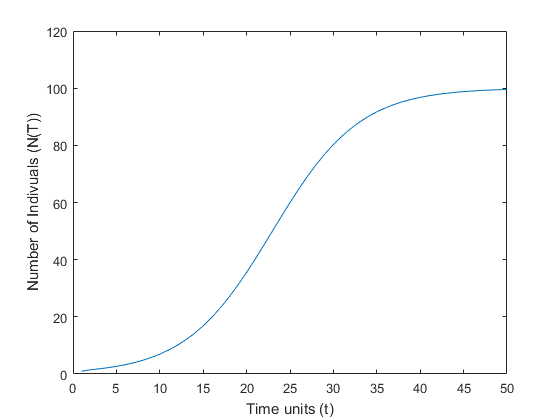
\includegraphics[width=\textwidth]{ContinousLogisticModel.png}
			\caption{Example of equation (60) where $N_0 = 1$ , $r=0.2$ , $k=100$ and maxium value of $t$ is 50}  
		\end{figure}
	
		As seen in equation 60 and visualised in figure 4 is that to begin with the population increases exponentially but as the it approaches the carrying capacity $K$ the population levels off. The population stops growing completely at the value $K$

		These trends show in figure 4 and equation 60  of models represent most typical populations and how they behave. But it is unwise to  assume populations will react in this way. One famous example of this was the prediction of 
		
		These types of models give us a model to understand how most populations grow. But you can not take it to a assume all models will behave in the same way. One example of this was the attempts to predict the population of the United States of America. Many predicted the population of the United States would level off in the 1940 (\cite{Peral}) much like figure 4 in this paper. But this did not happened and the population has until present day carried on to growing. This shows that it is not always possible to predict how a population will react over time.

	
		Looking at the previous model it can be noted that the population shown does not display trend that would be expected from a real world population. Mainly it can be  assumed that most populations will not reach a flat limit in growth and then stop growing. What would be expected would be a distortion when the population reaches its carrying capacity. This can behaviour can be explained by showing a small example of a population. Lets assume that a population every unit of time doubles in size and lets assume that the carrying capacity of the environment for the population equals 10. So starting with a population of 1 this example population will grow as so 1,2,4,8,16. As shown a population size of 16 exceeds the carry capacity of the environment so this must be dealt with. The previous model though does not show this behaviour. So a new  model just be developed.
	
		The simplest way to show this is a lag value in to the model.   
		\begin{equation}
		 \frac{dN}{dt}=rN(t)[1-\frac{N(t-T)}{K}] 
		\end{equation}
		In this equation $r$ is the rate in change. $N(t)$ is the number of individuals at point $t$ in time and $K$ is the carrying capacity. This means $T$ controls amount of lag that is occurring on the model.

		
		\begin{figure}[h!] 
			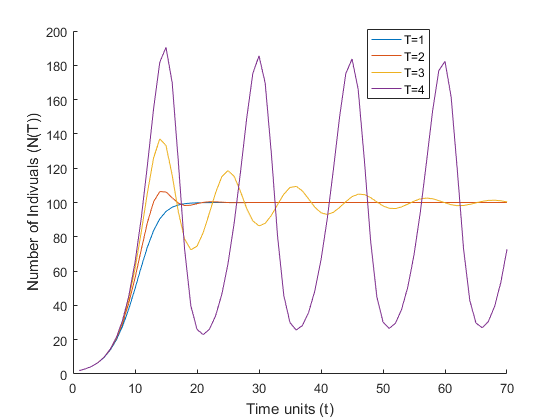
\includegraphics[width=\textwidth]{HutishingsonModel.png}
			\caption{Example of equation (61) where $N_0 = 2$ , $r=0.5$ , $k=100$ and maxium value of $t$ is 100. Also used are varying values of $T$}  
		\end{figure}
		
		Looking at figure 5 it can seen that number increasing the amount of lag ($T$) on the model causes the population to oscillate in increasing dramatic fashion around the carrying capacity $K$. In the lower $T$ values the population tends towards the carrying capacity on every oscillation but if the lag is great enough it causes the model to oscillate forever centred around the $K$ value. 
		
		\begin{table}[h!]

		\begin{tabular}[width=\textwidth]{ |p{3cm}||p{3cm}|p{3cm}|p{3cm}|p{3cm}|  }
			\hline
			$T$ Values& Peak of $N$ & After Reaching 100 once Minimum $N$ value& Rate of Rising to $K$ in units of $t$& Does Model Hold Oscillation Forever\\
			\hline
			T=1 &100   	&	NA 	&   NA &	No\\
			T=2 &106 	& 	98  &	9  &	No\\
			T=3 &137 	& 	72	&  	11 &	No\\
			T=4 &190 	& 	22	&  	15 &	Yes\\
			T=5 &270 	& 	0.3	&  	26 &	Yes\\
			T=6 &392 	& 	$-\infty$	&  	NA &	No\\
			T=7 &557 		& 	$-\infty$	&  	NA &	No\\
			T=8 &$3x10^{11}$ 	& 	$-\infty$	&  	NA &	No\\
			\hline
		\end{tabular}
		\caption{Table comparing values of $T$ when $N_0 = 2$ , $r=0.5$ , $k=100$}
		\end{table}
		
		Looking at table 3 is it clear to see that if the value $T$ is great enough the population becomes unstable causing the population to die out. This instability in this type of model is one of its major downsides.
		

	\subsubsection{Discrete Time Logistic models}

	The previous models show the how to make logistic models for continuous populations. But what of discrete populations. Below is a equation to model a logistic model for a discrete population. Where $K$ is the carrying capacity and $N_{t}$ is the number of individuals at time $t$ and $R$ is a rate of change.
	
	\begin{equation}
	 N_{t+1}=N_t+ RN_t(K-\frac{K-N_t}{K}) 
	\end{equation}
	
	\begin{figure}[h!] 
		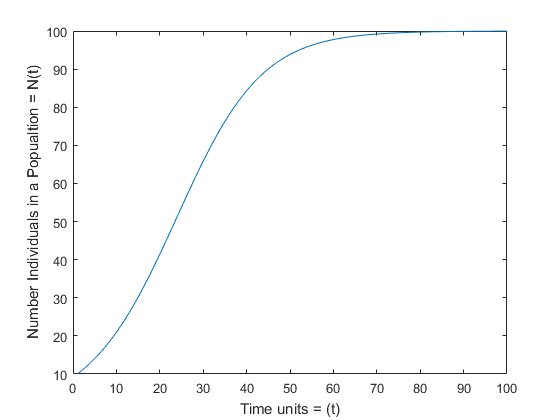
\includegraphics[width=\textwidth]{DiscreteLogisticModel.png}
		\caption{Example of equation (62) where starting population =1 0 , $R=0.5$ , $k=100$ and maximum value of $t$ is 100}  
	\end{figure}
	
	As you can see this graph is similar in results as equation 60 and this should be no surprise as they both modelling the same idea of limiting the population by a carrying capacity $K$. 
	
	\subsection{Simulation of a Single Population}
	
	Over the last section the idea of how  model a single type population of individual has been explored. These models can be tested and the trends and ideas shown by them can be looked in to by building a simulation.
	
	All the simulations shown will be using the assumption and ideas laid out in section 2 of the is paper(General Overview of Simulations Used). That section shows the basic layout of the simulations to be built.
	
	The first simulation that will be built is to help in the understanding of equitation 60. Due to being limited to a 2d grid the simulation will already have a a carrying capacity and this will be the size of the grid. This means that instead of food limiting the population it will be space. This will lead to slight difference in the results but the main goals of the simulation will stay the same as there is only one main limiting factor. 
	 
	So a simulation was designed that follow the basic rule set
	\begin{enumerate}
		\item A individual will never move from the cell it is born in to 
		\item An individual will have a 50\% chance each turn to breed
		\item A individual will reproduce in to a space above, below or left or right of the origin cell
		\item If the cell chosen to be reproduced in to is already filled by an  individual, the individual trying to reproduce will not be able to reproduce this turn
	\end{enumerate}
	
	I have implemented this rule set on a grid of size 100 by 100. This meant there was a carrying capacity on the population of 10000. 
	
	\begin{figure}[h!] 
		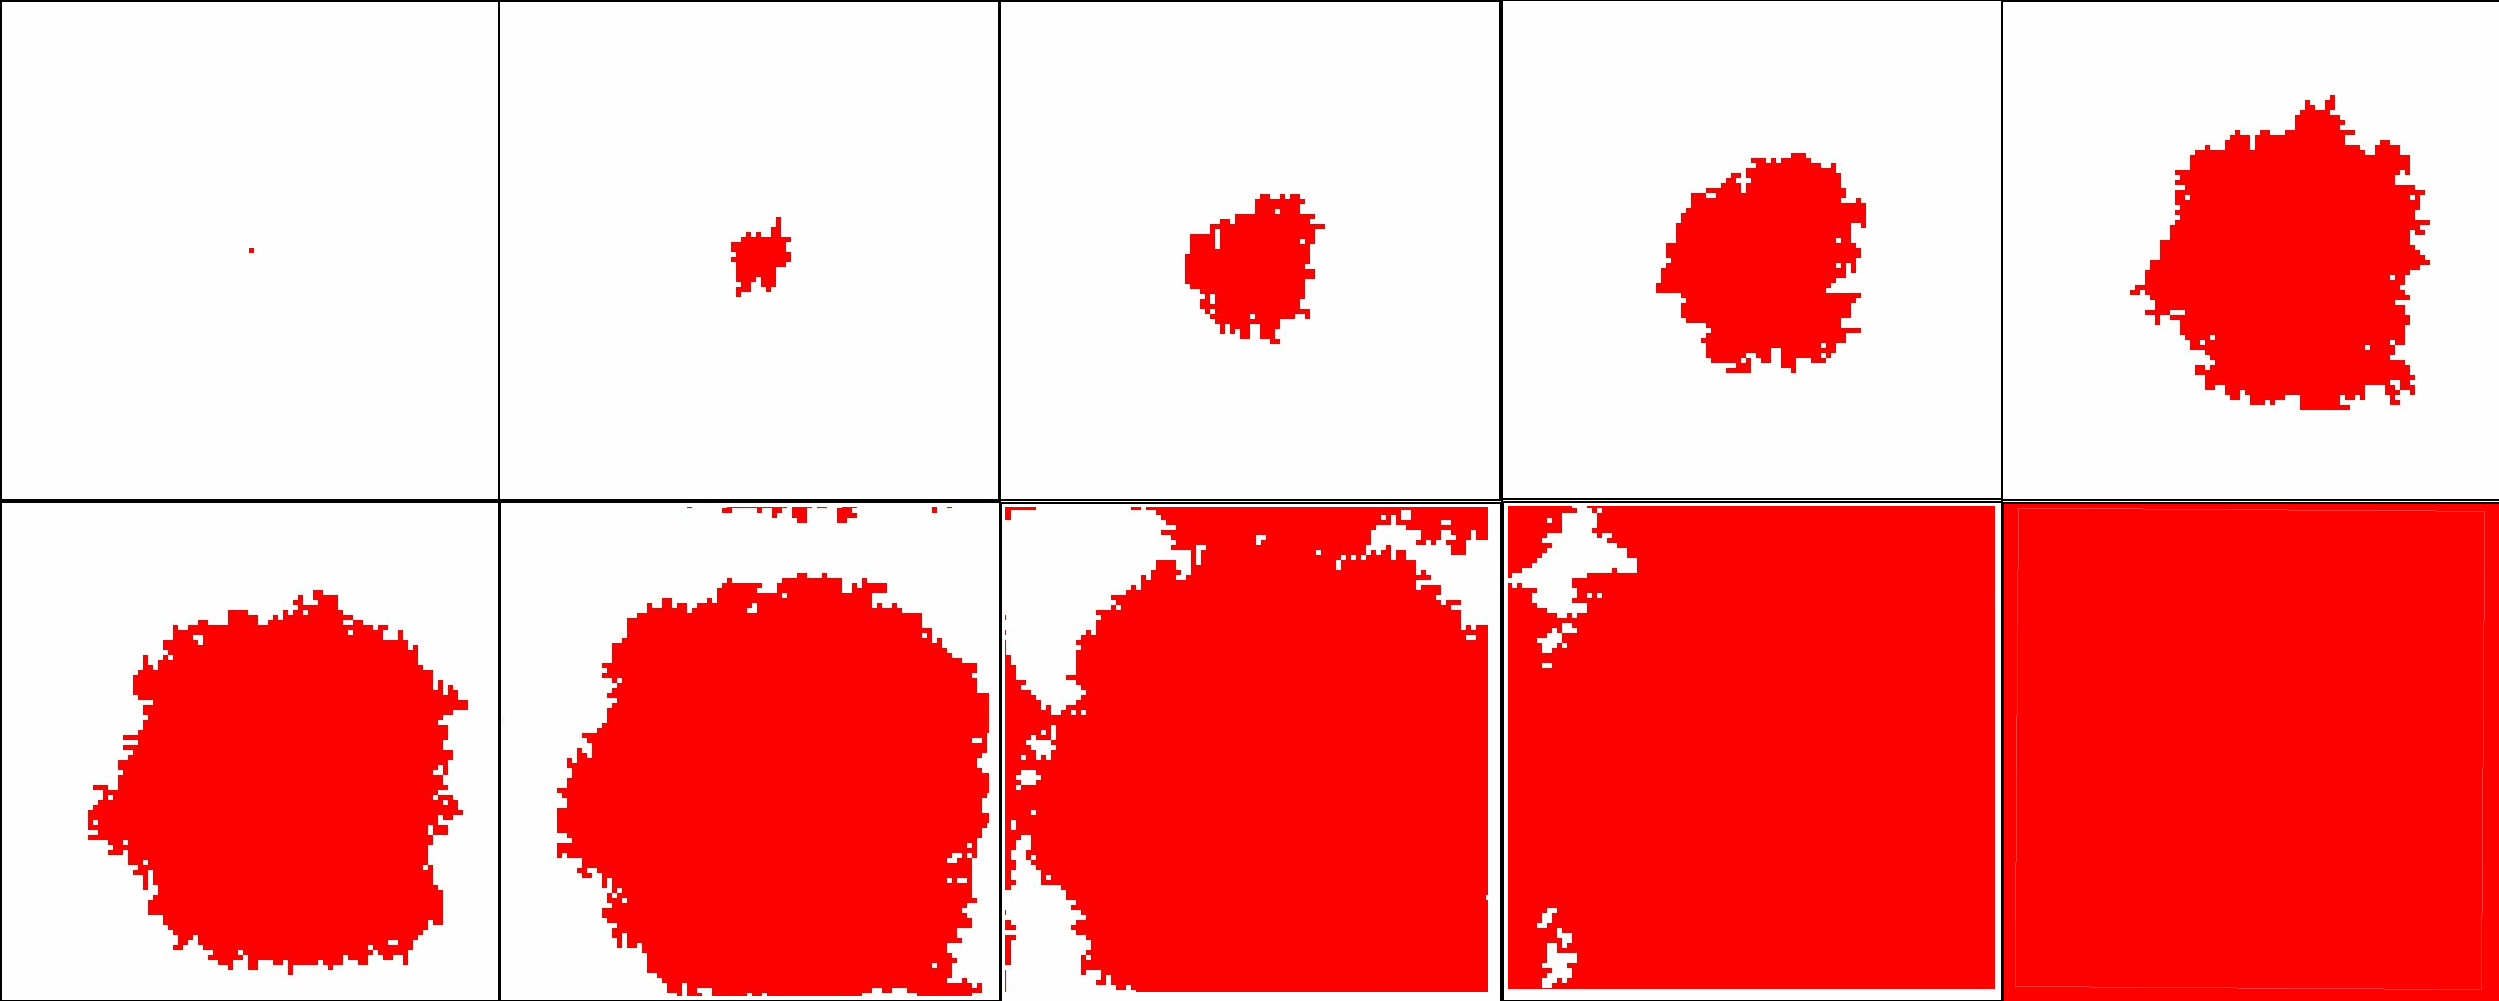
\includegraphics[width=\textwidth]{simulation1_1Collage.png}
		\caption{Figure shows simulation 1.1 at different states during its simulation. Starting top left and ending bottom right. the Images are at Turn 1, 25,50,75,100,125,150,175,200,225}  
	\end{figure}
	
	\begin{figure}[h!] 
		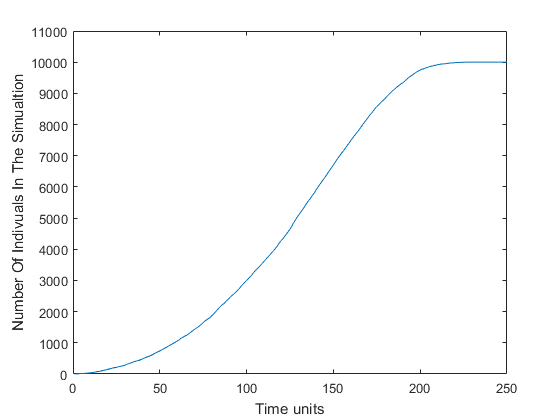
\includegraphics[width=\textwidth]{Simulation1GraphNumberIndivuals.png}
		\caption{Graph shows the amount of individuals in simulation 1.1 at certain time units}  
	\end{figure}
	
	As can be be seen from figure 7 and 8 the population of the simulation increased exponentially to begin with. But as the population neared the carrying capacity of the environment the growth rate of the population slowed down until it reached the carrying capacity at which point all growth stopped. It can be seen from figure 7 that the population grew out from the point of origin and expand out until in had filled the grid. 
	
	The conclusions that can be drawn from this simulation are that it compares very simlarity to equation 60 in its analysis of results. With figures 4 and 8 begin almost identical shape. From this it can be seen that these models and simulations are accurate as they both were made using to different methods and come from 2 separate sources.
	 
	
	This trend is an important to populations as it is a way of showing how they can grow and reach a maximum amount of individuals. This trend can be seen across a number of real world populations.
	
	The next step for this simulation will be to add death to the simulation. This was achieved by adding this rule
	
	If an individual is surrounded on 4 sides by non empty space the individual will die. 
	
	This rule was added to simulation 1.1 to produce simulation 1.2.
	
	\begin{figure}[h!] 
		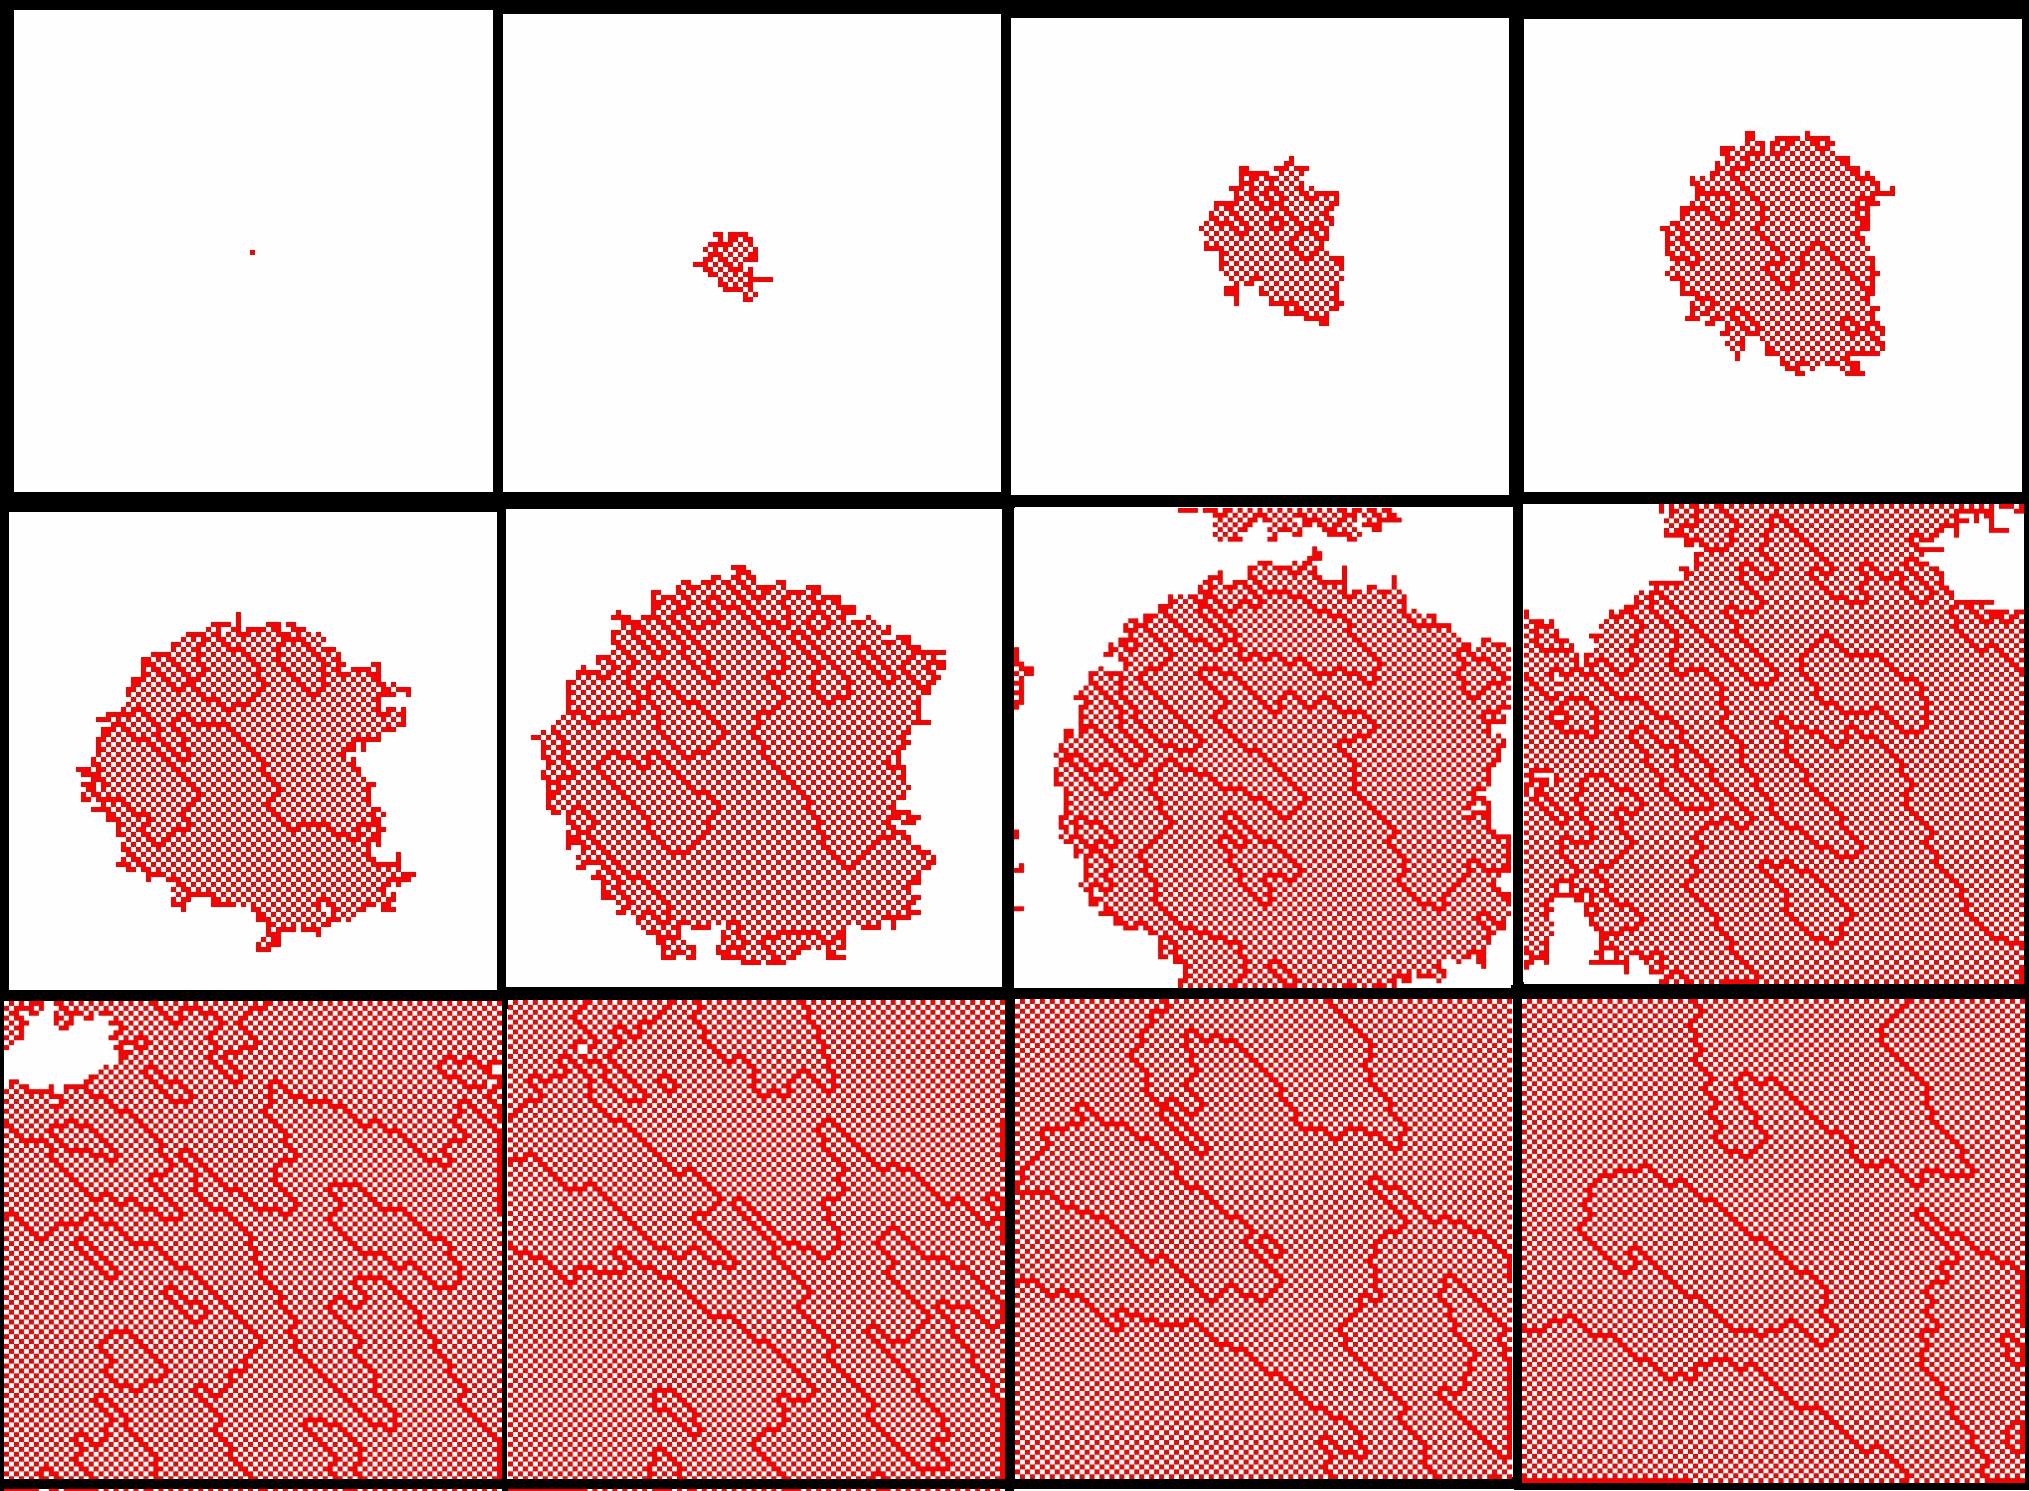
\includegraphics[width=\textwidth]{simulation1_2Collage.png}
		\caption{Figure shows simulation 1.2 at different states during the simulation. Starting top left and ending bottom right. the Images are at Turn 1, 25,50,75,100,125,150,175,200,225,250,275}  
	\end{figure}

	\begin{figure}[h!] 
		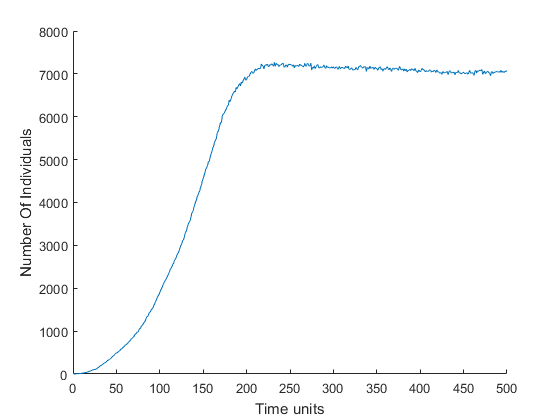
\includegraphics[width=\textwidth]{Simulation1_2GraphNumberIndivuals.png}
		\caption{Graph shows the amount of individuals in simulation 1.2 at certain time units}  
	\end{figure}

	It can be seen from figure 9 and 10 that simulation 1.2 behaves similarly to simulation 1.1. This shows us the that the trend observed from the previous simulation still hold true for this simulation. From this it can seen that adding in death does not change the trend seen in the population. But it can be seen that it does change the carrying capacity of the environment decreasing it by about 2500 individuals. Also it can be observed that as the population reaches a carrying capacity a amount of noise can be found distorting the line around this point.
	
	Also it can be observed that emergent behaviour can be seen from the simulation. Emergent behaviour means the whole population has properties that each individual does not have.In this case it can be seen that the individuals of the population from shapes and lines on the grid and then these shapes drift along the grid. This type of behaviour would not be able to be seen if the simulation was not visualised and the mathematical models do not display the behaviour.This is a clear advantage of using a simulation to show a population. This behaviour does also explain why there is noise on the line in figure 10 showing number of individuals as it reaches the carrying capacity. 
	
	The carrying capacity of this environment for this population can be found by finding the average of the noise affecting the number of individual present in the population once the simulation reaches a beyond a certain number of turns.
		
	\begin{table}[h!]
		\centering
		\caption{Table showing analysis of values from simulation 1.2}
		\begin{tabular}{|l|l|l|}
			\hline
			Turns Being Analysed &  Turn 220 to 250	&Turn 400 to 500 \\
			\hline
			Average Value        & 7203  		   	& 7043           \\
			Minimum Value        & 7116   			& 6955           \\
			Maximum Value        & 7269  			& 7131            \\
			\hline
		\end{tabular}
	\end{table}
	
	
	It can be seen from table 4 that at the peak of the number of individuals in the population is not the carrying capacity of the population but at the point just after the population has stopped expectationally growing. It can seen that type of behaviour is like the behaviour  shown in equation 61 where the population also grows above the carrying capacity of the environment. Explicitly this be can seen in figure 5 when $T=2$. This behaviour is also explained with in that section
	
	There is other factors to be explored about simulation 1.2. Firstly it can be seen that the later in the simulation the population mostly takes the from of a checkered grid unlike simulation 1.1 where it becomes a solid block. This happens due to the fact that even if these cells are bred in to by a member of the population they are killed immediately due to the death rule that has now been included.
	

\section{Multi population models}

	

	Multi population models are important because they show how populations of different populations interact with each other. This enables the analysis of how competition or exploitation and other cross population relationships. The first relationship  will be explored is competition between populations.
	
	\subsection{Competition}
		Competition is a very common feature in most populations. Competition is a relationship between many populations in which they are after a limited amount of a resource(eg food or space). This causes harm to the maximum size that the populations can reach.
		
		\subsubsection{Competition for Food} 
		
		One way to show competition between populations is a Lotka-Volterra models. Lotka-Volterra models are a simple extension of the logistic models looked at previously in this paper. (\cite{GAUSE44})
		
		Firstly a logistic model looks like equation (63)
		\begin{equation}
		\frac{dN}{dt} = rN(1-\frac{N}{K}) 
		\end{equation}
		
		Denoting $a_1 = \frac{1}{k}$ so that 

		\begin{equation}
		\frac{dN}{dt} = rN(1-a_1N) 
		\end{equation}
		
		But now to look at 2 populations competing for the same resource. So letting $N_i$ which is the number of individuals in species $i$ and $r_i$ the rate of growth for population $i$. Also 4 positive constants will be declared  $a_{ij}$ which is the effect of species $i$ on species $j$. From these figures the equation (65) and (66) can be denoted. 
		
		\begin{equation}
		\frac{dN_1}{dt} = r_1N_1(1-a_{11}N_1-a{12}N_2) 
		\end{equation}
		\begin{equation}
		\frac{dN_2}{dt} = r_2N_2(1-a_{21}N_1-a{12}N_2)  
		\end{equation}
		
		These equations can be rewritten as 
			\begin{equation}
			\frac{dN_1}{dt} = \frac{r_1N_1}{K_1}(K_1-N_1-a{12}N_2) 
			\end{equation}
			\begin{equation}
			\frac{dN_2}{dt} = \frac{r_2N_2}{K_2}(K_1-a{21}N_1-N_2) 
			\end{equation}
		so that $K$ is expressed explicitly which is often useful to do.

		\begin{figure}[h!] 
			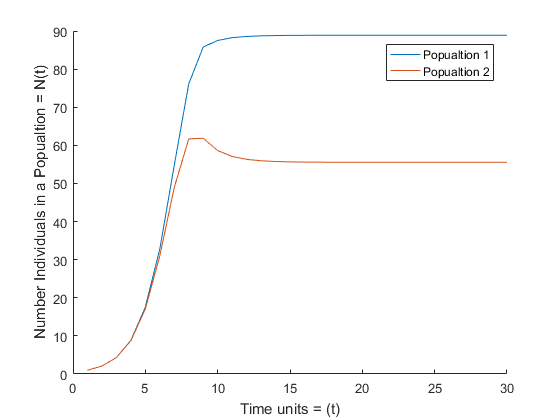
\includegraphics[width=\textwidth]{CompetitionForFood.png}
			\caption{A graph showing effects of equations (66),(67). Where the numbers are set as $N_1=1$, $N_2=1$, $r_1=1.1$, $r_2=1.1$, $K_1=100$, $K_2=100$, $a_{12}=0.2$, $a_{21}=0.5$  and $t$ goes to a maximum of 30
				}
		\end{figure}
		
		The equations (67) and (68)  can be plotted and this has been done in figure 11.As can be seen from figure 11 both populations grow at the same rate to begin with this is due to them both having the same $r$. Yet as both populations increase in size the rate of growth in population 2 slows down this is due to the fact it is being limited by the increasing size of population 1. This causes the a down turn in the size of population 2. Population 1 eventually reaches a set number of member of individuals in the population and so does population 2 though it worth noting in both populations they are limited to lower values than there carrying capacities.
		
	\subsubsection{Simulation Of Competition}
	
		A simulation can be built to show how competition can affect populations.This simulation follows the same rules as simulation 1.2 but it changes the start conditions so that it starts with 2 populations instead of 1 . Population 1 cells where set to have a 50\% chance of breeding every turn and population 2 with a 25\% chance of breeding every turn. This simulation will be called simulation 2 
		
		Competition in this simulation is not over food like in the previous examples but over space. This should produce a similar result in the simulation as it is model how if one resource is competed over by 2 populations.
		
		\begin{figure}[h!] 
			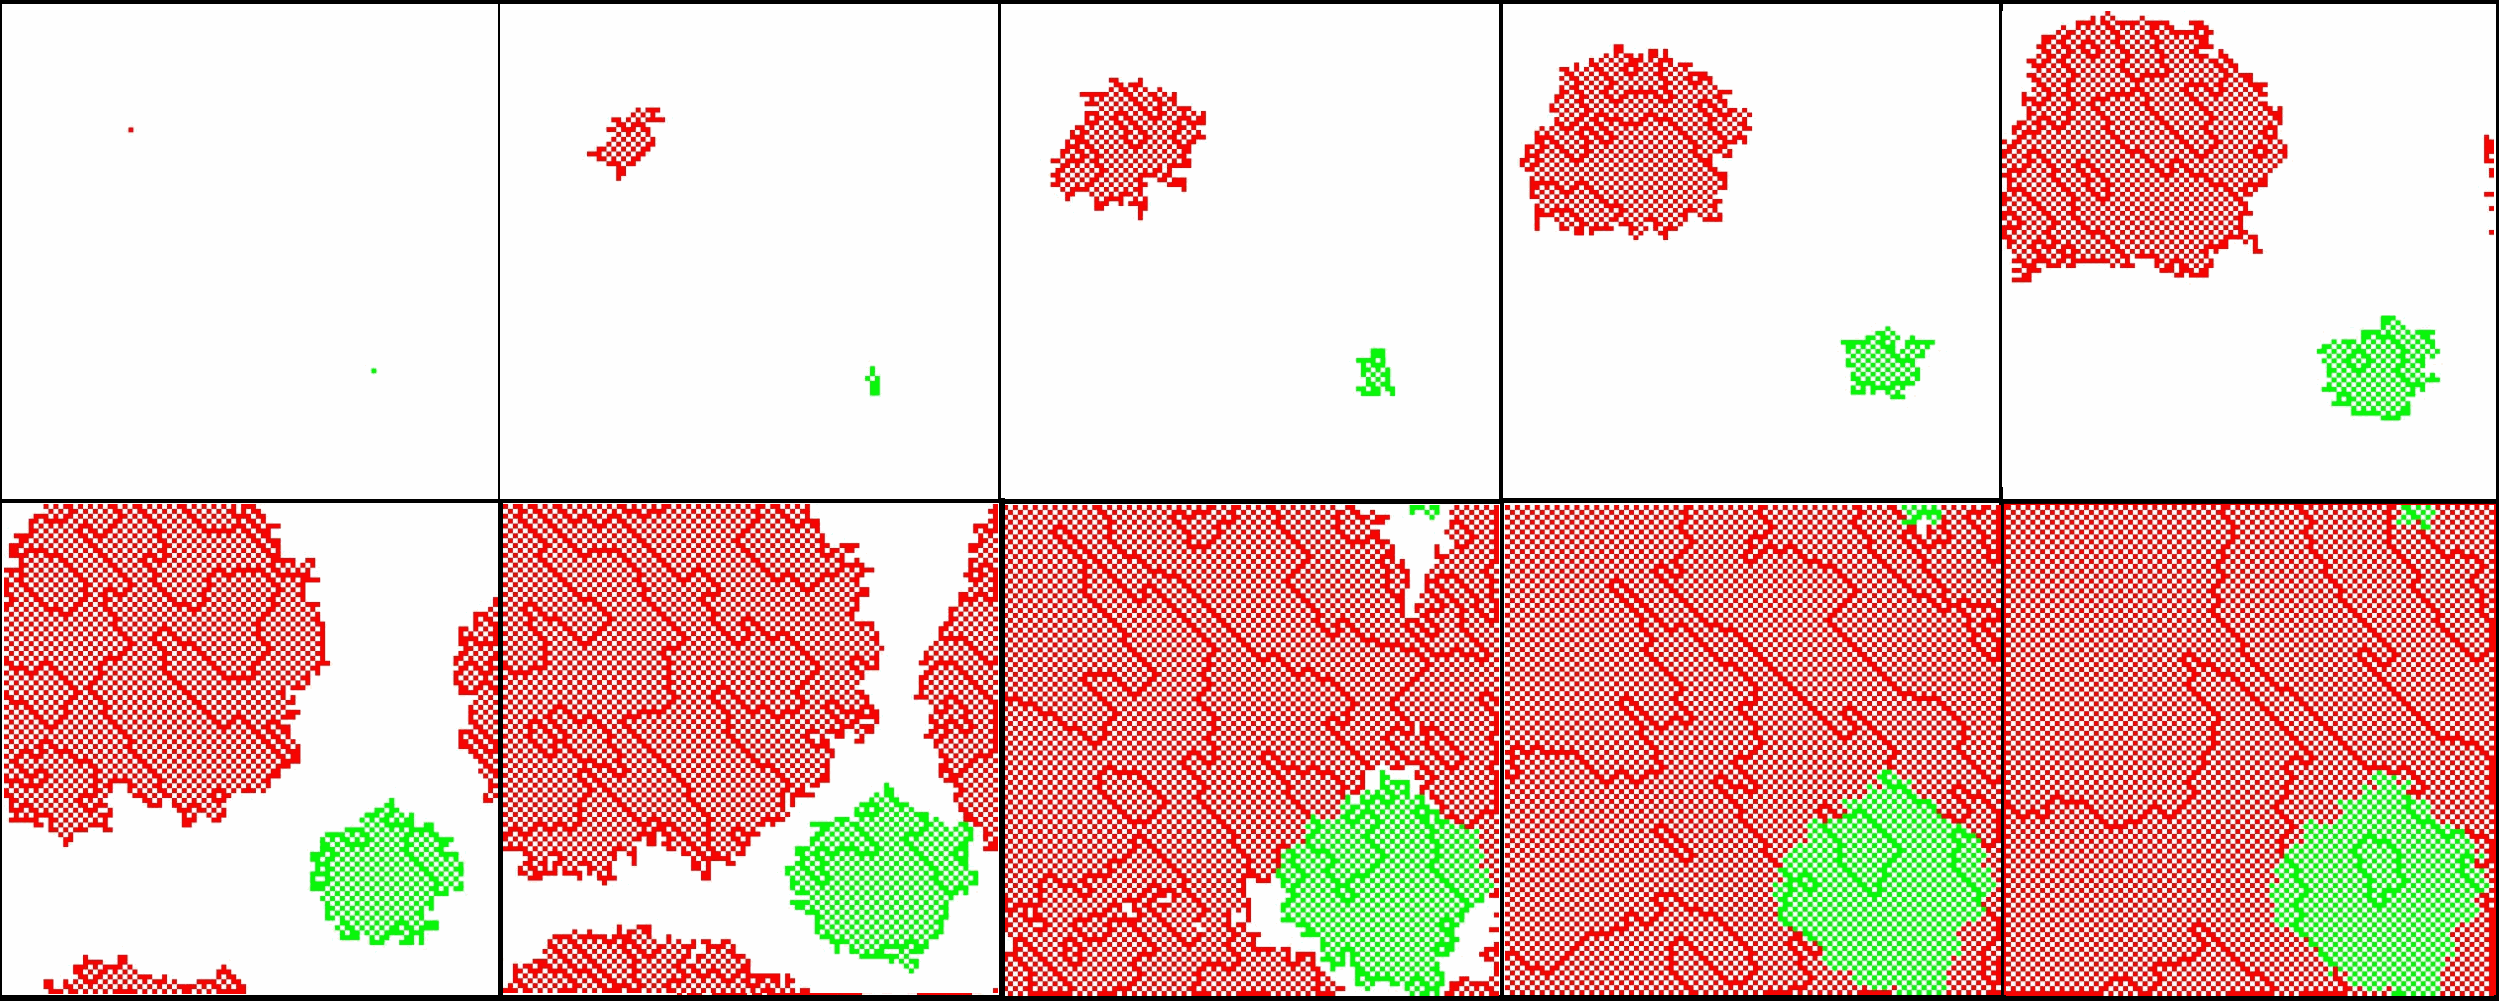
\includegraphics[width=\textwidth]{simulation2Collage.png}
			\caption{A series of pictures showing simulation 2 in action. Picture are of turns 1,25,50,75,100,125,150,175,200,225,250. Population 1 individuals are coloured red and population 2 individuals are coloured green}
		\end{figure}
		
		\begin{figure}[h!] 
			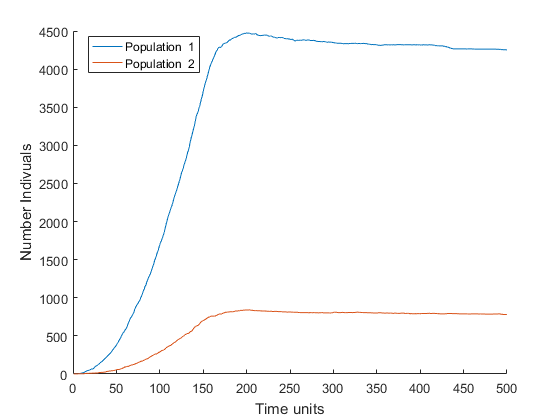
\includegraphics[width=\textwidth]{Simulation2GraphNumberInviduals.png}
			\caption{A graph showing number individuals in a population against time for simulation 1.2}
		\end{figure}
		
		As can be seen from this simulation if merely looking at one population it can be noted that see again the same dynamics as seen for simulation 1.2 . When examining figure 13 it can be noted that both populations rise at different rates and both raise to their carrying capacities. In both populations they raise past this capacities before lowering slightly to a value.
		
		It is also worth noting that emergent behaviour appears again in the simulation and it shows that the behaviour crosses over the 2 populations shown. This is to be expected as they both follow the same rule set 
		
		
		
	\subsection{Predator-Prey}
	Predator-Prey models are an important type of model. This is because they are one of the most common type of relationships between 2 species and they show unique and interesting dynamics that are not shown in many other population relationships. 
	
	\subsubsection{Lotka-Volterra model}
	Firstly to show predator prey models Lotka-Volterra models will be used as they have been used previously in this paper. But this time assumptions will made about the predator and prey populations

	\begin{itemize}
		\item Prey will grow exponential with out any predators present in the population.
		\item Predator with out prey present die off exponentially
		\item Prey being killed bys predator will be take the the form of a linear function
		\item Each prey death contributes to growth of the predator population 
	\end{itemize}
	
	From this it can be denoted that the number of individuals in the prey population denoted as $H$ and the number of individuals in the predator population as denoted as $P$ .It can be assumed that when $P=0$ that
	\begin{equation} 
	\frac{dH}{dt}=rH
	\end{equation}
	$r$ denoting the rate of increase of the number of prey when there are no predators present
	Secondly can also assumed that 
	\begin{equation} 
	 \frac{dP}{dt}=-kP 
	\end{equation}
	$k$ denoting the rate of decline of the number of predators when there are no prey present. 
	Thirdly can be assume that there must be a death rate for prey as they are eaten by the predator population . So with this $bHP$ can be said to equals the death rate.  Where $b$ represents a constant value that the predator population eats the prey population. So equation 69 can be expanded to.
	\begin{equation} 
	 \frac{dH}{dt}=rH-bHP
	\end{equation}
	Finally it was assumed that the predator population grows at constant rate for each prey killed so $cHP$ becomes the birth rate of the predator population where $c$ is a constant value relating to growth of predators relating to prey. So equation 70 can be expanded to.
	
	\begin{equation} 
	\frac{dP}{dt}=cHP-kP
	\end{equation} 
	
	\begin{figure}[h!] 
				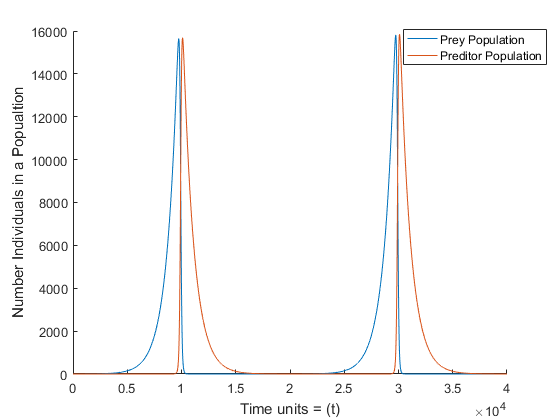
\includegraphics[width=\textwidth]{PredPreyModel.png} 
				\caption{A graph showing effects of equations (71),(72). Where 
					$r=b=c=k=1$ and starting populations of Prey and predator = $0.99$
					} 
	\end{figure}
	
	Firstly it can seen that the prey population in figure 14 increases exponentially but once it reaches a certain point the predictor population shoots up causing the prey population to drop rapidly. As the amount of prey has now drop this cause the predator population to drop rapidly. This process this then back to its starting position. As can be seen this means the populations oscillate. This can be proven in the model as a identical peaks can be seen later in the figure.
	
	
	\subsubsection{Adding Density Dependence}
	The important next step is to move from the above models to a model that has a density dependence that affects the prey population. This is a important feature as a environment can only support so many prey individuals. This can be added to the Lotka-Volterra models above to get
	

	\begin{equation}  \frac{dH}{dt}=rH[1-\frac{H}{K}]-bHP	\end{equation} 
	\begin{equation} \frac{dP}{dt}=cHP-kP \end{equation} 
	
	 \begin{figure}[h!] 
	 	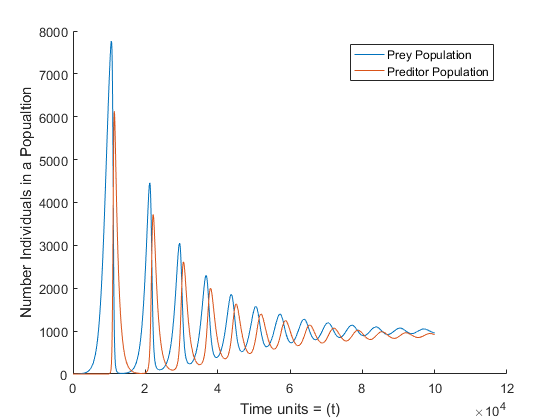
\includegraphics[width=\textwidth]{PredPreyDiscrete.png} 
	 	\caption{A graph showing effects of equations (75),(76). Where $r=b=c=k=1$ and starting populations of Prey and predator = $0.99$ and $K=10$
	 	} 
	 \end{figure}
	 
	 As can be seen from figure 15 is that the population dynamics seen are much like those seen in figure 14. Expect that every peak and trough gets closer to towards the carrying capacity of the prey population. This means both populations approach the carrying capacity of the  prey population.

	\subsubsection{Functional Response}
	
	It can be noted that some of the assumptions made previously are unrealistic. It can be seen that as the number of prey increases the rate prey is killed by the predators increases. But this rate cannot keep increasing forever. This is because predators in the real world cannot catch and kill a infinite amount of prey. This means there must be other limiting factors acting on the the populations causing the prey population to increase but the rate of prey killed to level off.  From this point on the the rate of prey killed will be defined as a function of the number of prey and predators present as a functional response.  
	
	
	This functional response can be added to the models above to get the equations


	\begin{equation} \frac{dH}{dt}=rH[1-\frac{H}{K}]-bf(H)P\end{equation} 
	\begin{equation} \frac{dP}{dt}=cf(H)P-kP \end{equation}  
	
	Where $f(H)$ represents the functional response.
	
	From the above models the equations below can be generated
	\begin{equation}rH[1-\frac{H}{K}]-bf(H)P = 0 \end{equation} 
	So solving this for $P$ gets you the equation
	\begin{equation} P = \frac{rH(1-\frac{H}{K})}{bf(H) }  \end{equation} 
	
	
	
	\subsection{Host-Parasitiod}
	A host-parasitiod relationship is one where the parasitiod lives in close association with a host 	and at the host's expense. The parasitiod at some point will kill the host. There are similarities between this type of relationship and Predator-Prey relationship. Though parasitiod are often very different than a predator as they usually actively need there hosts to  enable themselves to breed often killing the host in the process.This leads to a very close relationship between host and parasitiod
	
	
	\subsubsection{Nicholson-Bailey model}
	
	Firstly the number of hosts at a time $t$ will be defined as  $N_t$ and number of parasitiods at a time $t$ will be defined as $P_t$. As in a predator prey model it will be assumed that without any parasitiods the number of hosts will grow exponentially at a rate $\lambda$ per $t$ time unit. Also the function $f(N_T,P_t)$ will equal the probability of a host $N$  breeding with out being infected by parasitiod $P$. Also $c$ will be set as the amount of parasitiods born from all infected hosts. From these assumptions the equations (79) and (80) can be made.
	
	\begin{equation} N_{t+1}=\lambda N_tf(N_t,P_t) \end{equation} 
	\begin{equation} P_{t+1}=cN_t[1-f(N_t,P_t)] \end{equation} 
	 
	 
	 The next step is to decide on how to define $f(N_t,P_t)$. $f(N_t,P_t)$ shows the relationship between host and parasitiod density. Firstly it will be assumed that parasitiods search though a host population randomly and can lay unlimited eggs. This means what is being described is a distribution where the parasitiods are being put on a random hosts. This is like a Poisson distribution where you put place objects into random boxes. This means that the chance of a host not being infected by the parasitiods is the zero term on Poisson distribution. This get the equation (81)
	 
	\begin{equation} f=e^{-aP_t} \end{equation} 
	
	$a$ is the parameter that measures the efficiency of the parasitiod. This can be put in to formulas(79) and (80) to get the equations below.
	
	\begin{equation} N_{t+1}=\lambda N_te^{-aP_t} \end{equation} 
	\begin{equation} P_{t+1}=cN_t[1-e^{-aP_t}] \end{equation} 
	
	
	\begin{figure}[h!] 
		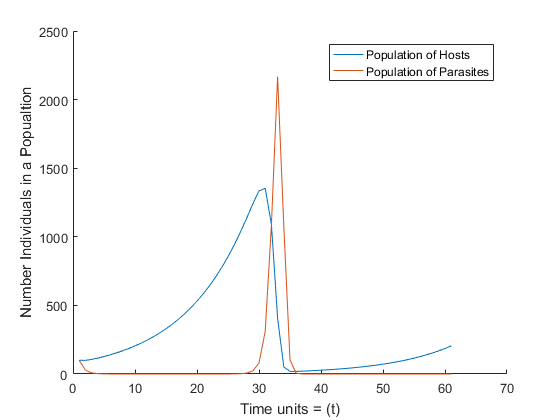
\includegraphics[width=\textwidth]{hostParasite.png} 
		\caption{ A graph showing effects of equations (84),(85). Where $a=0.001$ , $ \lamda =1.1$,$c=3$ and start populations for hosts and parasites is 100. }
			
	\end{figure}

	It can be seen from figure 16 that this relationship is very similar to that of a predator prey model. With the host growing exponentially to begin with and this causing a spike in the  amount of parasites. But it can be seen that this population is not stable as the number of parasites hit 0

	It can be proven that the equations 82 and 83 are not stable by getting the equilibrium of the equations. The equilibrium can be retrieved by setting $N=N_t=N_{t+1}$ and $P=P_t=P_{t+1}$.
	
	\begin{equation} N= \frac{\lambda ln(\lambda)}{(\lambda - 1)ac} \end{equation}
	\begin{equation} P=\frac{ln(\lambda)}{a} \end{equation}
	
	These equations can be used numerical to prove that this model is not stable under any starting conditions.

	\subsubsection{Stabilizing Features}
	Above we have seen that the host-parasitiod model we have presented is unstable. Where are several features that could be added that can be used to stabilise this model.
	\begin{itemize}
		\item Adding density dependence for the host 
		\item Adding a interference among parasitiods causing a lowering in the growth rate of parasitiods under certain conditions
		\item Creating a refuge for hosts so they could not be infected by the parasitiod
	\end{itemize}
	These concepts can be used to modify and improve the Nicholson-Bailey model and to increase stability in the model.
	
	
	
\section{Disease in a population}
	Another important feature that can be studied about a population is how disease effects them. Much like a host-parasitiod model is can be used to cause a population to stop growing at a exponential rate. Being investigated is how epidemics of disease can effect a population. Often disease epidemics happen in short time compared to hosts lifetime so population dynamics will be ignored for the hosts
	
	\subsection{Epidemic models}
	A epidemic is a widespread occurrence of an infectious disease over a particular time. The point of modelling this is to answer to major questions. Firstly epidemics tend to stop before population dies off. So are some of the population immune or is there another population dynamics reason? Secondly under what conditions will there be an epidemic happen?
	
	Firstly a size of the population will be declared as $N$. With $I,S,R$ being the sub-populations representing infected,susceptible and removed individuals.The infected population are defined as individuals who currently have the ability to infect others.The susceptible population is defined as individuals who do not have the disease currently but could potentially get the disease. Finally the removed population will be defined as individuals that have had the disease and now can no longer infect others.
	
	The total population size can be defined as 
	\begin{equation}N = I+S+R \end{equation} 
	
	It can be assumed that there is a rate of infection for the population proportional to the number of infected and susceptible sub populations. This will be defined as  $\beta SI$ where $\beta$ is the contact rate. There must also be a removal rate defined as $\gamma$. This denotes the rate at which the infected population turns in to the removed population. From these assumptions several equations can be defined.
	
	
	\begin{equation} \frac{dS}{dt} = - \beta SI  \end{equation} 
	
	\begin{equation} \frac{dI}{dt} = \beta SI - \gamma I \end{equation}
	
	\begin{equation} \frac{dR}{dt} = \gamma I\end{equation}
	
	\begin{figure}[h!] 
		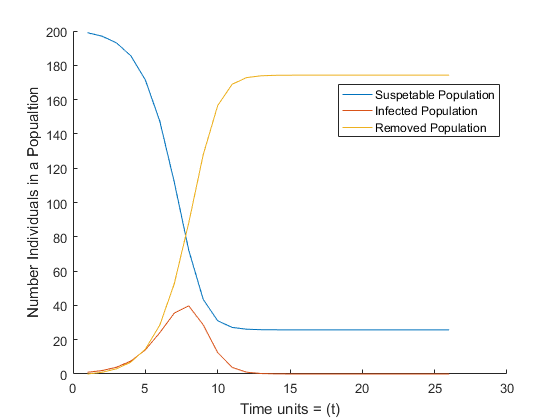
\includegraphics[width=\textwidth]{Epidmic.png} 
		\caption{ A graph showing effects of equations (86),(87), (88). Where $\gamma = 1$ and $\beta = 0.01$.And at $t=1$ $I=1$ $S=200$ and $R=0$}
	\end{figure}
	
	As can be seen from figure 17 the number of susceptible of individuals drops exponentially this causes the infected and removed populations to quickly grow. though it is worth noting both populations are growing roughly the same rate. Eventually the rate of infection levels off but the rate of removal does not causing the amount of infected to drop to 0 with this the removed population stops growing. This leaves with only the susceptible population and removed population with individuals in them.
		
	This answers one of the questions asked at the start of this section are some of the population immune or is there another population dynamics reason for why some of a population are not effected by a epidemic? Figure 17 proves that it is due to a population dynamic reason. To analysis why this is the equilibrium will be found for these equations.
		
		
		
	So lets set $\frac{dS}{dt} = 0 $ and $\frac{dI}{dt} = 0$. From this it can be seen that the number of infected ($I$) must be 0 but the value of $S$ can vary. Also the infected population has no chance of increasing in size as soon as the size of the infected population equals 0. This means for an endemic disease (as population dynamics for the hosts has been ignored) has no chance of staying at a steady level in a population. 
		
	But what of the second question	what conditions will there be an epidemic happen? Well firstly $\frac{dI}{dt} > 0$ so this means that 
	
	\begin{equation}\beta SI - \gamma I>0\end{equation}
	
	This can be divided by $I$ to get 
	\begin{equation}\beta S - \gamma >0\end{equation}
	
	This can rearrange into
	\begin{equation}R_0=\frac{\beta S}{\gamma} >1\end{equation}
	
	Where $R_0$ is the reproductive number of the disease. This is important as $R_0$ shows the mean number of new infections caused by a single infected individual. $\beta S$ shows the rate an infected individual causes new infections. While $\frac{1}{\gamma}$ is the mean time an individual is infected. From this it be can deuced that if  $R_0$ is greater than 1 then the incidents of the disease will increase  and if $R_0$ less than 1 incidents of the disease will decrease. For this last statement this gives the knowledge required to get the minimum population size needed to cause an epidemic. With the maximum size of susceptible individuals being the total population size at the start of a epidemic means the equations below can be generated.
	
	\begin{equation} \frac{\beta N}{\gamma} >1\end{equation}
	\begin{equation} N>\frac{\gamma}{\beta}\end{equation}
	
	This can be seen as accurate as there is much evidence to support this theory that a minimum population size is needed to cause an epidemic.

	Now that the start of the epidemic has been investigated what of the end of a epidemic.
	
	At start epidemic number of infected is almost zero. So at the end of epidemic this is also true. So at end of epidemic will number susceptible individuals equal zero? In figure 17 it has proved this is not the case but can it be proved mathematically.
	\begin{equation}\frac{dI}{dS}= -1 + \frac{\gamma}{\beta S}	\end{equation}
	
	\begin{equation}dI= [-1 + \frac{\gamma}{\beta S}]dS	\end{equation}
	This can be integrated so that 
	\begin{equation}I= -S + \frac{\gamma}{\beta }ln(S)+C	\end{equation}
	Using the knowledge that has been learned  about the start of an epidemic so it can be assumed that $I=0$ and $S=N$ so 
	\begin{equation}0= \frac{\gamma}{\beta }ln(N)-N+C\end{equation}
	\begin{equation} C=-\frac{\gamma}{\beta }ln(N)+N \end{equation}
	
	$C$ can be added in to equation (98).
	\begin{equation}I= \frac{\gamma}{\beta }ln(S)-\frac{\gamma}{\beta }ln(N)-N+S\end{equation}
	
	At end of epidemic know number of infected is 0 so
	\begin{equation}0= \frac{\gamma}{\beta }ln(S)-\frac{\gamma}{\beta }ln(N)-N+S\end{equation}
	
	To solve this equation to find $S$ is quite difficult. But knowing enough information about the solution it can be proved that $S$ must be greater than 0. As if $S=N$ the right hand side of the equation = 0 and as $S$ approaches 0 the right hand side of the equation goes to negative infinity. So from this S must be greater than 0 this is proved also by first in McKendrik (\cite{Kermack700}). This knowledge backs up the results from figure 17.
	
	\section{Conclusion}
	In conclusion it can seen that though out this paper many population dynamics have been discussed and analysed. These population trends are important as if they can affect one population it is very likely they will affect other populations as well. This makes the simple populations that have been modelled and simulated useful as the dynamics seen within them can be used to understand and explain how real world populations react.
	
	It was assumed that the simplest population to model and demonstrate would be a single population that has no limits applied to it. This lead to the making of a density independent model. It can be seen by analysing  these dynamics show that populations would grow exponentially in this model. This model was then expanded upon by investigating how the age of a individual  would affect a population. These models made exploring this could be expanded upon as only on as the models produced only dealt with populations with a very short life span in terms of generations overlapping. This means that these models can be explored further by having models that show populations with long life spans and seeing how the they compare. All these previous population models have had no limitations placed upon them so a model was developed that explored how these limit on populations can affect the dynamics.
	
	
	This lead to the creation of the density dependant models. These models showed how a population would react if a limit was placed on them. It was seen that these models would expand to there limit but as soon as got close to it there rate of growth would slow down. A simulation was also made for this model. This dynamic could be investigated further by having this limit change over time and seeing what affect this would have on the population. Also what if multiple limits where affecting the population how would this affect the growth of the population? These areas of population dynamics could be investigated further. 
	
	The previous models all revolved around the dynamics of one population on itself but what of 2 population that interact with each other. This lead to the development of several models that explore the various relationships that can occur between populations.
	
	First the idea of competition between populations was explored. This type of relationship is quite common in nature as many species often compete other the same food resource. So models where made to show this. Like the density dependant models shown before it can seen that the populations will raise in size until they reach a limit. This limit due to this competitions was lower than the limit shown for the single population model. This type of model was also simulated.These models could be further expand upon by changing the dynamic of the competition over time and changing the overall limit of the environment the populations are in.
	
	Secondly the idea of predator and prey populations was explored. This is also another type of population that appears commonly in nature. These models lead to a dynamic that caused oscillations in the populations.  These models where also developed with some quite big assumptions made upon them but though out the section many ways are suggested at dealing with these assumptions. These ways such as functional response and  including density dependence for prey could be explored further. This could lead to a better understanding of these oscillations and the dynamics as a whole.
	
	Thirdly the idea of a host-parasitiod relationship was explored. This type of population is far less common than previous relationships between populations but is still a important relationship to understand. This relationship showed a similar dynamic to the predator and prey populations expect that the model made was unstable in nature. This relationship could be explored further by exploring the methods suggested at the end of the section that suggest ways to stabilise the this relationship between host and parasitiod.
	
	The last section covered is how disease effects a population.It also explored how a disease could spread though out a population and how this could be modelled. This section also dealt with how to show a epidemic could occur in a population. These models could be expanded upon to show how a population would deal with a prolonged disease affecting it(Eg flu every winter).
	
	Though out the paper simulations are used to show the populations in action. These simulations follow a general set of limitations. The simulations could be investigated further by changing these limitations such as having the simulations run on a 3d grid instead of a 2d grid and seeing the affects this has on the simulations. The simulations could also be used to run on different starting conditions and slight variations on the rule sets. This would help in the understanding and results drawn from the rule sets used.
	
	As can be seen there is still much to be discussed about population dynamics. But this paper has shown the basics in populations and how there dynamics can be modelled and explained. Both mathematically and though the use of simulations.
	

	\bibliography{bib}
	
\end{document}


